% Created by tikzDevice version 0.10.1 on 2016-09-02 12:02:26
% !TEX encoding = UTF-8 Unicode
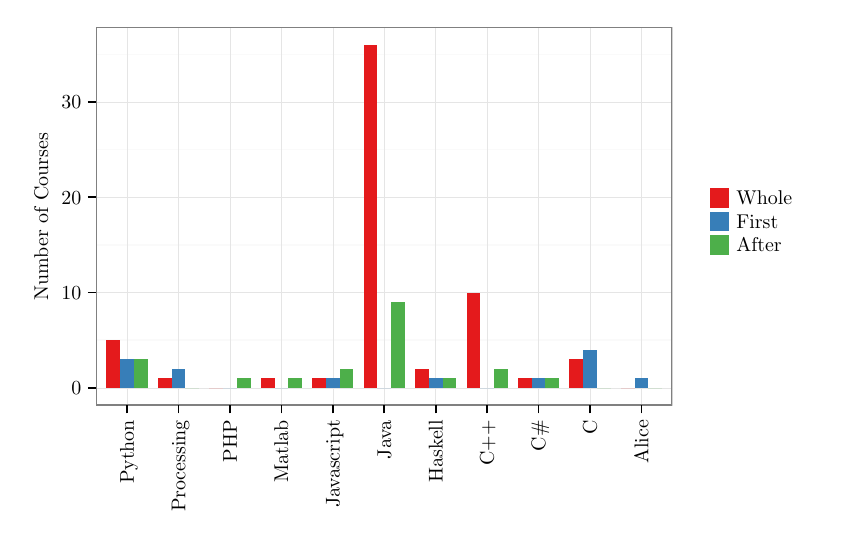
\begin{tikzpicture}[x=1pt,y=1pt]
\definecolor{fillColor}{RGB}{255,255,255}
\path[use as bounding box,fill=fillColor,fill opacity=0.00] (0,0) rectangle (289.08,180.67);
\begin{scope}
\path[clip] (  0.00,  0.00) rectangle (289.08,180.67);
\definecolor{drawColor}{RGB}{255,255,255}
\definecolor{fillColor}{RGB}{255,255,255}

\path[draw=drawColor,line width= 0.6pt,line join=round,line cap=round,fill=fillColor] (  0.00,  0.00) rectangle (289.08,180.68);
\end{scope}
\begin{scope}
\path[clip] ( 24.76, 44.28) rectangle (232.93,180.67);
\definecolor{fillColor}{RGB}{255,255,255}

\path[fill=fillColor] ( 24.76, 44.28) rectangle (232.93,180.67);
\definecolor{drawColor}{gray}{0.98}

\path[draw=drawColor,line width= 0.6pt,line join=round] ( 24.76, 67.70) --
	(232.93, 67.70);

\path[draw=drawColor,line width= 0.6pt,line join=round] ( 24.76,102.15) --
	(232.93,102.15);

\path[draw=drawColor,line width= 0.6pt,line join=round] ( 24.76,136.59) --
	(232.93,136.59);

\path[draw=drawColor,line width= 0.6pt,line join=round] ( 24.76,171.03) --
	(232.93,171.03);
\definecolor{drawColor}{gray}{0.90}

\path[draw=drawColor,line width= 0.2pt,line join=round] ( 24.76, 50.48) --
	(232.93, 50.48);

\path[draw=drawColor,line width= 0.2pt,line join=round] ( 24.76, 84.92) --
	(232.93, 84.92);

\path[draw=drawColor,line width= 0.2pt,line join=round] ( 24.76,119.37) --
	(232.93,119.37);

\path[draw=drawColor,line width= 0.2pt,line join=round] ( 24.76,153.81) --
	(232.93,153.81);

\path[draw=drawColor,line width= 0.2pt,line join=round] ( 35.91, 44.28) --
	( 35.91,180.67);

\path[draw=drawColor,line width= 0.2pt,line join=round] ( 54.50, 44.28) --
	( 54.50,180.67);

\path[draw=drawColor,line width= 0.2pt,line join=round] ( 73.08, 44.28) --
	( 73.08,180.67);

\path[draw=drawColor,line width= 0.2pt,line join=round] ( 91.67, 44.28) --
	( 91.67,180.67);

\path[draw=drawColor,line width= 0.2pt,line join=round] (110.26, 44.28) --
	(110.26,180.67);

\path[draw=drawColor,line width= 0.2pt,line join=round] (128.85, 44.28) --
	(128.85,180.67);

\path[draw=drawColor,line width= 0.2pt,line join=round] (147.43, 44.28) --
	(147.43,180.67);

\path[draw=drawColor,line width= 0.2pt,line join=round] (166.02, 44.28) --
	(166.02,180.67);

\path[draw=drawColor,line width= 0.2pt,line join=round] (184.61, 44.28) --
	(184.61,180.67);

\path[draw=drawColor,line width= 0.2pt,line join=round] (203.20, 44.28) --
	(203.20,180.67);

\path[draw=drawColor,line width= 0.2pt,line join=round] (221.78, 44.28) --
	(221.78,180.67);
\definecolor{fillColor}{RGB}{228,26,28}

\path[fill=fillColor] ( 28.47, 50.48) rectangle ( 33.43, 67.70);
\definecolor{fillColor}{RGB}{55,126,184}

\path[fill=fillColor] ( 33.43, 50.48) rectangle ( 38.39, 60.81);
\definecolor{fillColor}{RGB}{77,175,74}

\path[fill=fillColor] ( 38.39, 50.48) rectangle ( 43.34, 60.81);
\definecolor{fillColor}{RGB}{228,26,28}

\path[fill=fillColor] ( 47.06, 50.48) rectangle ( 52.02, 53.93);
\definecolor{fillColor}{RGB}{55,126,184}

\path[fill=fillColor] ( 52.02, 50.48) rectangle ( 56.98, 57.37);
\definecolor{fillColor}{RGB}{77,175,74}

\path[fill=fillColor] ( 56.98, 50.48) rectangle ( 61.93, 50.48);
\definecolor{fillColor}{RGB}{228,26,28}

\path[fill=fillColor] ( 65.65, 50.48) rectangle ( 70.61, 50.48);
\definecolor{fillColor}{RGB}{55,126,184}

\path[fill=fillColor] ( 70.61, 50.48) rectangle ( 75.56, 50.48);
\definecolor{fillColor}{RGB}{77,175,74}

\path[fill=fillColor] ( 75.56, 50.48) rectangle ( 80.52, 53.93);
\definecolor{fillColor}{RGB}{228,26,28}

\path[fill=fillColor] ( 84.24, 50.48) rectangle ( 89.19, 53.93);
\definecolor{fillColor}{RGB}{55,126,184}

\path[fill=fillColor] ( 89.19, 50.48) rectangle ( 94.15, 50.48);
\definecolor{fillColor}{RGB}{77,175,74}

\path[fill=fillColor] ( 94.15, 50.48) rectangle ( 99.11, 53.93);
\definecolor{fillColor}{RGB}{228,26,28}

\path[fill=fillColor] (102.82, 50.48) rectangle (107.78, 53.93);
\definecolor{fillColor}{RGB}{55,126,184}

\path[fill=fillColor] (107.78, 50.48) rectangle (112.74, 53.93);
\definecolor{fillColor}{RGB}{77,175,74}

\path[fill=fillColor] (112.74, 50.48) rectangle (117.69, 57.37);
\definecolor{fillColor}{RGB}{228,26,28}

\path[fill=fillColor] (121.41, 50.48) rectangle (126.37,174.48);
\definecolor{fillColor}{RGB}{55,126,184}

\path[fill=fillColor] (126.37, 50.48) rectangle (131.32, 50.48);
\definecolor{fillColor}{RGB}{77,175,74}

\path[fill=fillColor] (131.32, 50.48) rectangle (136.28, 81.48);
\definecolor{fillColor}{RGB}{228,26,28}

\path[fill=fillColor] (140.00, 50.48) rectangle (144.95, 57.37);
\definecolor{fillColor}{RGB}{55,126,184}

\path[fill=fillColor] (144.95, 50.48) rectangle (149.91, 53.93);
\definecolor{fillColor}{RGB}{77,175,74}

\path[fill=fillColor] (149.91, 50.48) rectangle (154.87, 53.93);
\definecolor{fillColor}{RGB}{228,26,28}

\path[fill=fillColor] (158.59, 50.48) rectangle (163.54, 84.92);
\definecolor{fillColor}{RGB}{55,126,184}

\path[fill=fillColor] (163.54, 50.48) rectangle (168.50, 50.48);
\definecolor{fillColor}{RGB}{77,175,74}

\path[fill=fillColor] (168.50, 50.48) rectangle (173.46, 57.37);
\definecolor{fillColor}{RGB}{228,26,28}

\path[fill=fillColor] (177.17, 50.48) rectangle (182.13, 53.93);
\definecolor{fillColor}{RGB}{55,126,184}

\path[fill=fillColor] (182.13, 50.48) rectangle (187.09, 53.93);
\definecolor{fillColor}{RGB}{77,175,74}

\path[fill=fillColor] (187.09, 50.48) rectangle (192.04, 53.93);
\definecolor{fillColor}{RGB}{228,26,28}

\path[fill=fillColor] (195.76, 50.48) rectangle (200.72, 60.81);
\definecolor{fillColor}{RGB}{55,126,184}

\path[fill=fillColor] (200.72, 50.48) rectangle (205.67, 64.26);
\definecolor{fillColor}{RGB}{77,175,74}

\path[fill=fillColor] (205.67, 50.48) rectangle (210.63, 50.48);
\definecolor{fillColor}{RGB}{228,26,28}

\path[fill=fillColor] (214.35, 50.48) rectangle (219.30, 50.48);
\definecolor{fillColor}{RGB}{55,126,184}

\path[fill=fillColor] (219.30, 50.48) rectangle (224.26, 53.93);
\definecolor{fillColor}{RGB}{77,175,74}

\path[fill=fillColor] (224.26, 50.48) rectangle (229.22, 50.48);
\definecolor{drawColor}{gray}{0.50}

\path[draw=drawColor,line width= 0.6pt,line join=round,line cap=round] ( 24.76, 44.28) rectangle (232.93,180.67);
\end{scope}
\begin{scope}
\path[clip] (  0.00,  0.00) rectangle (289.08,180.67);
\definecolor{drawColor}{RGB}{0,0,0}

\node[text=drawColor,anchor=base east,inner sep=0pt, outer sep=0pt, scale=  0.72] at ( 19.36, 48.00) {0};

\node[text=drawColor,anchor=base east,inner sep=0pt, outer sep=0pt, scale=  0.72] at ( 19.36, 82.45) {10};

\node[text=drawColor,anchor=base east,inner sep=0pt, outer sep=0pt, scale=  0.72] at ( 19.36,116.89) {20};

\node[text=drawColor,anchor=base east,inner sep=0pt, outer sep=0pt, scale=  0.72] at ( 19.36,151.33) {30};
\end{scope}
\begin{scope}
\path[clip] (  0.00,  0.00) rectangle (289.08,180.67);
\definecolor{drawColor}{RGB}{0,0,0}

\path[draw=drawColor,line width= 0.6pt,line join=round] ( 21.76, 50.48) --
	( 24.76, 50.48);

\path[draw=drawColor,line width= 0.6pt,line join=round] ( 21.76, 84.92) --
	( 24.76, 84.92);

\path[draw=drawColor,line width= 0.6pt,line join=round] ( 21.76,119.37) --
	( 24.76,119.37);

\path[draw=drawColor,line width= 0.6pt,line join=round] ( 21.76,153.81) --
	( 24.76,153.81);
\end{scope}
\begin{scope}
\path[clip] (  0.00,  0.00) rectangle (289.08,180.67);
\definecolor{drawColor}{RGB}{0,0,0}

\path[draw=drawColor,line width= 0.6pt,line join=round] ( 35.91, 41.28) --
	( 35.91, 44.28);

\path[draw=drawColor,line width= 0.6pt,line join=round] ( 54.50, 41.28) --
	( 54.50, 44.28);

\path[draw=drawColor,line width= 0.6pt,line join=round] ( 73.08, 41.28) --
	( 73.08, 44.28);

\path[draw=drawColor,line width= 0.6pt,line join=round] ( 91.67, 41.28) --
	( 91.67, 44.28);

\path[draw=drawColor,line width= 0.6pt,line join=round] (110.26, 41.28) --
	(110.26, 44.28);

\path[draw=drawColor,line width= 0.6pt,line join=round] (128.85, 41.28) --
	(128.85, 44.28);

\path[draw=drawColor,line width= 0.6pt,line join=round] (147.43, 41.28) --
	(147.43, 44.28);

\path[draw=drawColor,line width= 0.6pt,line join=round] (166.02, 41.28) --
	(166.02, 44.28);

\path[draw=drawColor,line width= 0.6pt,line join=round] (184.61, 41.28) --
	(184.61, 44.28);

\path[draw=drawColor,line width= 0.6pt,line join=round] (203.20, 41.28) --
	(203.20, 44.28);

\path[draw=drawColor,line width= 0.6pt,line join=round] (221.78, 41.28) --
	(221.78, 44.28);
\end{scope}
\begin{scope}
\path[clip] (  0.00,  0.00) rectangle (289.08,180.67);
\definecolor{drawColor}{RGB}{0,0,0}

\node[text=drawColor,rotate= 90.00,anchor=base east,inner sep=0pt, outer sep=0pt, scale=  0.72] at ( 38.39, 38.88) {Python};

\node[text=drawColor,rotate= 90.00,anchor=base east,inner sep=0pt, outer sep=0pt, scale=  0.72] at ( 56.98, 38.88) {Processing};

\node[text=drawColor,rotate= 90.00,anchor=base east,inner sep=0pt, outer sep=0pt, scale=  0.72] at ( 75.56, 38.88) {PHP};

\node[text=drawColor,rotate= 90.00,anchor=base east,inner sep=0pt, outer sep=0pt, scale=  0.72] at ( 94.15, 38.88) {Matlab};

\node[text=drawColor,rotate= 90.00,anchor=base east,inner sep=0pt, outer sep=0pt, scale=  0.72] at (112.74, 38.88) {Javascript};

\node[text=drawColor,rotate= 90.00,anchor=base east,inner sep=0pt, outer sep=0pt, scale=  0.72] at (131.33, 38.88) {Java};

\node[text=drawColor,rotate= 90.00,anchor=base east,inner sep=0pt, outer sep=0pt, scale=  0.72] at (149.91, 38.88) {Haskell};

\node[text=drawColor,rotate= 90.00,anchor=base east,inner sep=0pt, outer sep=0pt, scale=  0.72] at (168.50, 38.88) {C++};

\node[text=drawColor,rotate= 90.00,anchor=base east,inner sep=0pt, outer sep=0pt, scale=  0.72] at (187.09, 38.88) {C\#};

\node[text=drawColor,rotate= 90.00,anchor=base east,inner sep=0pt, outer sep=0pt, scale=  0.72] at (205.67, 38.88) {C};

\node[text=drawColor,rotate= 90.00,anchor=base east,inner sep=0pt, outer sep=0pt, scale=  0.72] at (224.26, 38.88) {Alice};
\end{scope}
\begin{scope}
\path[clip] (  0.00,  0.00) rectangle (289.08,180.67);
\definecolor{drawColor}{RGB}{0,0,0}

\node[text=drawColor,rotate= 90.00,anchor=base,inner sep=0pt, outer sep=0pt, scale=  0.72] at (  7.36,112.48) {Number of Courses};
\end{scope}
\begin{scope}
\path[clip] (  0.00,  0.00) rectangle (289.08,180.67);
\definecolor{fillColor}{RGB}{255,255,255}

\path[fill=fillColor] (241.47, 93.60) rectangle (280.54,131.36);
\end{scope}
\begin{scope}
\path[clip] (  0.00,  0.00) rectangle (289.08,180.67);
\definecolor{fillColor}{RGB}{228,26,28}

\path[fill=fillColor] (246.45,115.65) rectangle (253.56,122.76);
\end{scope}
\begin{scope}
\path[clip] (  0.00,  0.00) rectangle (289.08,180.67);
\definecolor{fillColor}{RGB}{55,126,184}

\path[fill=fillColor] (246.45,107.12) rectangle (253.56,114.23);
\end{scope}
\begin{scope}
\path[clip] (  0.00,  0.00) rectangle (289.08,180.67);
\definecolor{fillColor}{RGB}{77,175,74}

\path[fill=fillColor] (246.45, 98.58) rectangle (253.56,105.69);
\end{scope}
\begin{scope}
\path[clip] (  0.00,  0.00) rectangle (289.08,180.67);
\definecolor{drawColor}{RGB}{0,0,0}

\node[text=drawColor,anchor=base west,inner sep=0pt, outer sep=0pt, scale=  0.72] at (256.08,116.73) {Whole};
\end{scope}
\begin{scope}
\path[clip] (  0.00,  0.00) rectangle (289.08,180.67);
\definecolor{drawColor}{RGB}{0,0,0}

\node[text=drawColor,anchor=base west,inner sep=0pt, outer sep=0pt, scale=  0.72] at (256.08,108.19) {First};
\end{scope}
\begin{scope}
\path[clip] (  0.00,  0.00) rectangle (289.08,180.67);
\definecolor{drawColor}{RGB}{0,0,0}

\node[text=drawColor,anchor=base west,inner sep=0pt, outer sep=0pt, scale=  0.72] at (256.08, 99.66) {After};
\end{scope}
\end{tikzpicture}
